\section{DESENVOLVIMENTO}

\subsection{Especificação das funcionalidades}

As funcionalidades foram organizadas por ator e verificadas na interface, nos hooks, nos contratos das Edge Functions e nas migrações do banco de dados. A classificação distingue o que possui fluxo de uso completo do que existe apenas como suporte técnico.

\begin{table}[htbp]
\centering
\caption{Funcionalidades e situação da implementação.}
\label{tab:funcionalidades}
\scriptsize
\begin{tabularx}{\textwidth}{>{\RaggedRight\arraybackslash}p{1.7cm}Y>{\RaggedRight\arraybackslash}p{4.0cm}}
\toprule
\textbf{Ator} & \textbf{Funcionalidade} & \textbf{Situação} \\
\midrule
Prestador & Cadastro e login por e-mail & Implementada \\
Prestador & Perfil, slug público e fuso horário & Implementada \\
Prestador & Grupos de horários, dias e faixas de atendimento & Implementada \\
Prestador & Agenda diária e estados dos compromissos & Implementada \\
Prestador & Bloqueio, horário extra, liberação e cancelamento & Implementada \\
Prestador & Avisos, Web Push e instalação como PWA & Implementada; entrega requer configuração e worker operacional \\
Prestador & Listagem de clientes & Parcial: API e hook existem; não há tela dedicada \\
Cliente & Acesso por link, seleção de data e horário & Implementada \\
Cliente & Reserva com nome, e-mail e telefone, sem conta & Implementada \\
Cliente & Confirmação por e-mail e cancelamento por token & Implementada; envio requer worker operacional \\
\bottomrule
\end{tabularx}
\fontepropria
\end{table}

\subsubsection{Fluxo do prestador}

Após autenticar-se, o prestador configura nome público, endereço curto e fuso horário. Em seguida, cria um grupo de disponibilidade, seleciona dias da semana e informa o início, a duração e a quantidade de atendimentos de cada faixa. A agenda diária reúne horários livres, bloqueios e reservas. Um intervalo específico pode ser bloqueado ou liberado sem alterar toda a recorrência; uma reserva pode ser cancelada, mas não apagada.

\subsubsection{Fluxo do cliente}

O cliente abre o link do prestador, escolhe uma data e um dos horários calculados pelo backend, preenche seus dados de contato e confirma. A API volta a validar a disponibilidade durante a transação, evitando que a seleção feita na tela seja tratada como garantia de reserva. O e-mail resultante contém o resumo e um link de cancelamento associado a token próprio.

\subsubsection{Registro visual da aplicação}

O fluxo de uso é representado por duas telas principais: a configuração de disponibilidade pelo prestador e a seleção de horários na página pública de reserva. Essas interfaces ilustram as funcionalidades centrais da Agendinha.

\begin{figure}[htbp]
    \centering

    \begin{minipage}[t]{0.47\textwidth}
        \centering
        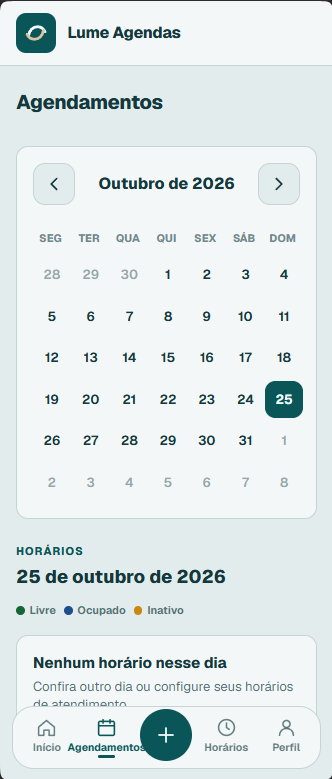
\includegraphics[
            width=\linewidth,
            height=6cm,
            keepaspectratio
        ]{agendinha-prestador.png}

        \caption{Configuração de horários do prestador.}
        \label{fig:tela-prestador}
    \end{minipage}
    \hfill
    \begin{minipage}[t]{0.47\textwidth}
        \centering
        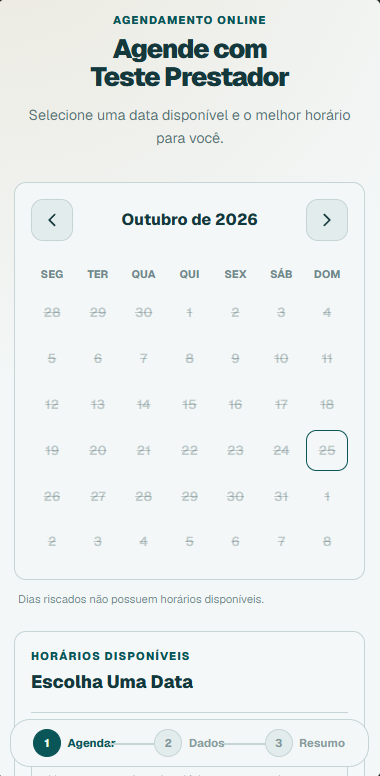
\includegraphics[
            width=\linewidth,
            height=6cm,
            keepaspectratio
        ]{agendinha-cliente.png}

        \caption{Seleção de horários pelo cliente.}
        \label{fig:tela-cliente}
    \end{minipage}
\end{figure}

Uma demonstração contínua dos fluxos da aplicação está disponível no \href{https://drive.google.com/drive/folders/1Iy3Y8jWdIG8WkwKIMk8nMqgSO8XAoJEi?usp=sharing}{vídeo de demonstração da Agendinha}.

\subsubsection{Critério de simplicidade}

Simplicidade não é medida apenas pelo número de telas. O desenho reduz decisões: o cliente não escolhe plano, não instala aplicativo e não cria senha; o prestador não precisa configurar infraestrutura. A avaliação exploratória, apresentada na Seção~\ref{sec:avaliacao}, permitiu verificar preliminarmente como essa redução se converte em tarefas concluídas e quais dificuldades permanecem.

\subsection{Arquitetura e fluxos do sistema}

A aplicação foi organizada em cliente web, serviços de backend, persistência e provedores especializados. A Figura~\ref{fig:arquitetura} apresenta os atores, componentes e serviços efetivamente utilizados pela Agendinha. As regras de domínio não dependem do estado local da tela: passam pelas Edge Functions, que coordenam autenticação, dados, cache e comunicação.

\begin{figure}[htbp]
    \centering
    \resizebox{\textwidth}{!}{\begin{tikzpicture}[
    font=\scriptsize,
    caixa/.style={draw=LumeAzul,fill=LumeClaro,rounded corners,minimum width=2.55cm,minimum height=1.35cm,align=center},
    servico/.style={draw=LumeVerde,fill=LumeMenta,rounded corners,minimum width=2.75cm,minimum height=1.35cm,align=center},
    dado/.style={draw=black!65!black,fill=black!8,rounded corners,minimum width=2.75cm,minimum height=1.35cm,align=center},
    seta/.style={-{Stealth[length=2mm]},LumeAzul,thick}
]
\node[caixa] (prestador) at (0,2.2) {\textbf{Prestador}\\painel autenticado};
\node[servico] (cliente) at (0,-0.2) {\textbf{Cliente}\\link público};
\node[caixa] (pwa) at (4,1) {\textbf{Next.js / PWA}\\React + TypeScript\\service worker};
\node[caixa] (auth) at (8,3) {\textbf{Supabase Auth}\\login + JWT};
\node[servico] (edge) at (8,1) {\textbf{Edge Functions}\\regras de negócio};
\node[dado] (postgres) at (8,-1) {\textbf{PostgreSQL}\\fonte oficial + RLS};
\node[caixa] (blackis) at (12,3) {\textbf{Upstash Redis}\\cache temporário};
\node[servico] (resend) at (12,1) {\textbf{Resend}\\e-mail};
\node[dado] (push) at (12,-1) {\textbf{Web Push}\\avisos};

\draw[seta] (prestador) -- (pwa);
\draw[seta] (cliente) -- (pwa);
\draw[seta] (pwa) -- node[above,sloped]{autentica} (auth);
\draw[seta] (pwa) -- node[above]{HTTPS} (edge);
\draw[seta] (edge) -- node[right]{SQL} (postgres);
\draw[seta] (edge) -- node[above,sloped]{cache} (blackis);
\draw[seta] (edge) -- node[above]{outbox} (resend);
\draw[seta] (edge) -- node[above,sloped]{avisos} (push);

\node[align=center,font=\scriptsize] at (6,-2.25) {Páginas: Network-First; recursos estáticos: cache local.\\Falha do Redis: consulta direta ao PostgreSQL.};
\end{tikzpicture}
}
    \caption{Arquitetura implementada da Agendinha.}
    \label{fig:arquitetura}
    \fontepropria
\end{figure}

\subsubsection{Atores, frontend e PWA}

A caixa \textbf{Prestador} representa o usuário autenticado que administra perfil, disponibilidade, exceções e compromissos. A caixa \textbf{Cliente} representa quem acessa o link público, consulta horários, reserva e cancela sem possuir conta. Ambos utilizam a mesma aplicação \textbf{Next.js/PWA}, construída com React e TypeScript, mas seguem rotas, permissões e contratos distintos.

O manifesto permite instalar a aplicação, e o service worker aplica Network-First às navegações para priorizar conteúdo atualizado e oferecer uma página de contingência quando não há conexão. Recursos estáticos elegíveis usam cache local; rotas de autenticação não são armazenadas. A interface pode registrar a inscrição do navegador para receber notificações Web Push quando o prestador concede permissão.

\subsubsection{Autenticação e regras de negócio}

O \textbf{Supabase Auth} mantém a identidade do prestador, oferece cadastro por e-mail e autenticação com Google e emite o JWT usado nas operações privadas. A interface não recebe credenciais administrativas. As \textbf{Edge Functions} validam entradas e origem, identificam o prestador, aplicam limites às rotas públicas e executam os casos de uso por meio de consultas e funções transacionais do banco.

Operações privadas combinam a validação do JWT com políticas de Row Level Security. Operações públicas, como consulta de disponibilidade e reserva, recebem validação específica e não expõem acesso irrestrito às tabelas. Esse desenho mantém a autorização no servidor, mesmo quando a interface antecipa validações para melhorar a experiência de preenchimento.

\subsubsection{Dados, cache e comunicações}

O \textbf{PostgreSQL} é a fonte oficial do estado de perfis, regras, clientes e reservas. Chaves estrangeiras, verificações, transações, RLS e a restrição de exclusão de intervalos protegem a consistência. O \textbf{Upstash Redis} mantém apenas disponibilidade derivada e controles auxiliares. As chaves incorporam o prestador, a data, a versão do esquema de cache e a versão da agenda; o TTL é configurável entre 10 e 900 segundos, com padrão de 60 segundos. Falhas de leitura ou gravação no Redis não interrompem a consulta ao banco.

O \textbf{Resend} transporta e-mails de confirmação e cancelamento. O \textbf{Web Push} entrega avisos de novas reservas e cancelamentos aos navegadores inscritos. Nenhum desses provedores participa da transação principal: eventos são gravados nas tabelas de outbox e consumidos por workers. Tentativas, falhas e reagendamentos permanecem registrados, de forma que uma indisponibilidade de comunicação não invalida uma reserva já confirmada.

\subsubsection{Fluxos críticos e tratamento de falhas}

A Figura~\ref{fig:fluxos} reúne a consulta de disponibilidade e a criação da reserva. Os fluxos conectam as caixas da arquitetura e mostram por que o cache acelera leituras, mas não substitui a validação transacional no PostgreSQL.

\begin{figure}[htbp]
    \centering
    \resizebox{\textwidth}{!}{\begin{tikzpicture}[
    font=\scriptsize,
    ator/.style={draw=LumeAzul!35,fill=LumeClaro,rounded corners,minimum width=1.6cm,minimum height=0.65cm,align=center},
    vida/.style={gray!55,dashed},
    msg/.style={-{Stealth[length=1.8mm]},LumeAzul,thick},
    msgb/.style={-{Stealth[length=1.8mm]},LumeVerde,thick}
]
\node[font=\bfseries] at (2.8,0.5) {A. CONSULTA DE DISPONIBILIDADE};
\node[ator] (c1) at (0,0) {Cliente};
\node[ator] (e1) at (2,0) {Edge};
\node[ator] (r1) at (4,0) {Redis};
\node[ator] (p1) at (6,0) {Postgres};
\foreach \x in {0,2,4,6}{\draw[vida] (\x,-0.35) -- (\x,-5.7);}
\draw[msg] (0,-0.8) -- node[above]{GET slots} (2,-0.8);
\draw[msg] (2,-1.5) -- node[above]{GET chave} (4,-1.5);
\draw[msg] (4,-2.2) -- node[above]{hit: dados} (2,-2.2);
\draw[msg] (2,-3.0) -- node[above]{miss: consulta} (6,-3.0);
\draw[msg] (6,-3.7) -- node[above]{dados oficiais} (2,-3.7);
\draw[msg] (2,-4.4) -- node[above]{SET + TTL} (4,-4.4);
\draw[msg] (2,-5.1) -- node[above]{horários} (0,-5.1);

\draw[gray!50] (7,-0.4) -- (7,-5.7);
\node[font=\bfseries] at (10.6,0.5) {B. RESERVA E CONFIRMAÇÃO};
\node[ator] (c2) at (8,0) {Cliente};
\node[ator] (e2) at (10,0) {Edge};
\node[ator] (p2) at (12,0) {Postgres};
\node[ator] (w2) at (14,0) {Workers};
\foreach \x in {8,10,12,14}{\draw[vida] (\x,-0.35) -- (\x,-5.7);}
\draw[msgb] (8,-0.8) -- node[above]{POST + chave} (10,-0.8);
\draw[msgb] (10,-1.6) -- node[above]{RPC transacional} (12,-1.6);
\node[draw=LumeVerde,minimum width=0.45cm,minimum height=0.45cm] at (12.25,-2.35) {};
\node[right] at (12.55,-2.35) {valida e bloqueia};
\node[draw=LumeVerde,minimum width=0.45cm,minimum height=0.45cm] at (12.25,-3.0) {};
\node[right] at (12.55,-3.0) {agenda + outbox};
\draw[msgb] (12,-3.7) -- node[above]{commit} (10,-3.7);
\draw[msgb] (10,-4.4) -- node[above]{confirmação} (8,-4.4);
\draw[msgb] (14,-5.1) -- node[above]{consome outbox} (12,-5.1);
\end{tikzpicture}
}
    \caption{Consulta de disponibilidade e criação de reserva.}
    \label{fig:fluxos}
    \fontepropria
\end{figure}

Na consulta, o cliente solicita um dia ou período pelo frontend. A Edge Function identifica o perfil pelo slug e busca no Redis as chaves correspondentes à versão corrente da agenda. Em um acerto, os horários validados são devolvidos sem nova leitura do PostgreSQL. Em uma ausência ou falha do Redis, o backend calcula os intervalos com base nos grupos ativos, regras semanais, exceções, reservas confirmadas e fuso horário. O resultado é devolvido mesmo sem cache e, quando possível, armazenado com TTL para consultas seguintes.

Na reserva, a Edge Function valida slug, intervalo, nome, e-mail, telefone e chave de idempotência. A função transacional volta a conferir se o período pertence à disponibilidade, normaliza os dados do cliente, mantém o vínculo com o prestador e tenta inserir o agendamento. A restrição de exclusão no PostgreSQL decide conflitos concorrentes: somente uma das solicitações pode manter o mesmo intervalo confirmado. A resposta da operação é vinculada à chave de idempotência para impedir duplicidade em reenvios.

Na mesma transação são criados o agendamento e os eventos necessários às outboxes. Depois do commit, a versão da agenda no Redis é incrementada, tornando obsoletas as chaves anteriores sem depender de sua remoção imediata. A resposta de sucesso retorna ao cliente antes do envio das mensagens. Workers separados reivindicam registros pendentes, chamam Resend e Web Push e registram sucesso, falha ou nova tentativa. Assim, erros no cache ou nos provedores de comunicação degradam recursos auxiliares, mas não alteram a decisão de integridade tomada pelo banco.

\subsection{Persistência e integridade dos dados}

\todoe{Melhorar a descrição da camada de persistência.}

A persistência separa disponibilidade recorrente, exceções, identidade dos clientes, reservas e suporte operacional. O esquema é definido por migrações SQL e utiliza tipos nativos do PostgreSQL, chaves estrangeiras, unicidade, verificações de intervalo e políticas de acesso. A Figura~\ref{fig:der} apresenta as onze tabelas persistentes na versão documentada, com tipos, chaves e cardinalidades.

O perfil estende a identidade administrada pelo Supabase Auth. Cada perfil possui grupos de horários, e cada grupo reúne regras por dia da semana. A duração do atendimento e a quantidade de horários são armazenadas na regra, enquanto exceções representam bloqueios ou disponibilidade adicional. A separação entre \texttt{Client} e \texttt{ProviderClient} permite reutilizar a identidade do cliente e preservar os dados informados no relacionamento com cada prestador.


\begin{figure}
\thispagestyle{fancy}
\vspace*{-0.6cm}
\noindent\begin{minipage}[t]{\linewidth}
\captionsetup{hypcap=false}
\captionof{figure}{Diagrama entidade-relacionamento da Agendinha.}
\label{fig:der}
\centering
\resizebox{1\linewidth}{!}{\begin{tikzpicture}[
    font=\scriptsize,
    entidade/.style={draw=black!80,fill=white,inner sep=2pt,align=left,anchor=north west},
    rel/.style={-{Stealth[length=1.5mm]},black!70,thin},
    rotulo/.style={fill=white,inner sep=1pt,font=\scriptsize}
]

\node[entidade] (profiles) at (0,0) {
\begin{tabular}{@{}lll@{}}
\rowcolor{black!15}\multicolumn{3}{c}{\textbf{profiles}}\\
PK/FK & \texttt{id} & uuid\\
 & \texttt{name} & text\\
UQ & \texttt{public\_slug} & text\\
 & \texttt{phone} & text?\\
 & \texttt{timezone} & text\\
 & \texttt{updated\_at} & timestamptz
\end{tabular}};

\node[entidade] (groups) at (6.4,0) {
\begin{tabular}{@{}lll@{}}
\rowcolor{black!15}\multicolumn{3}{c}{\textbf{AvailabilityRuleGroup}}\\
PK & \texttt{id} & uuid\\
FK & \texttt{provider\_id} & uuid\\
 & \texttt{name} & text\\
 & \texttt{is\_active} & boolean
\end{tabular}};

\node[entidade] (rules) at (13,0) {
\begin{tabular}{@{}lll@{}}
\rowcolor{black!15}\multicolumn{3}{c}{\textbf{AvailabilityRule}}\\
PK & \texttt{id} & uuid\\
FK & \texttt{group\_id} & uuid\\
 & \texttt{day\_of\_week} & smallint\\
 & \texttt{start\_time} & time\\
 & \texttt{end\_time} & time\\
 & \texttt{slot\_duration\_minutes} & smallint\\
 & \texttt{appointment\_count} & smallint
\end{tabular}};

\node[entidade] (idempotency) at (20.4,0) {
\begin{tabular}{@{}lll@{}}
\rowcolor{black!15}\multicolumn{3}{c}{\textbf{idempotency\_record}}\\
PK & \texttt{operation} & text\\
PK & \texttt{idempotency\_key} & uuid\\
 & \texttt{request\_hash} & text\\
 & \texttt{response} & jsonb\\
 & \texttt{created\_at} & timestamptz
\end{tabular}};

\node[entidade] (overrides) at (0,-4.8) {
\begin{tabular}{@{}lll@{}}
\rowcolor{black!15}\multicolumn{3}{c}{\textbf{AvailabilityOverride}}\\
PK & \texttt{id} & uuid\\
FK & \texttt{provider\_id} & uuid\\
 & \texttt{start\_datetime} & timestamptz\\
 & \texttt{end\_datetime} & timestamptz\\
 & \texttt{is\_available} & boolean
\end{tabular}};

\node[entidade] (clients) at (6.4,-4.8) {
\begin{tabular}{@{}lll@{}}
\rowcolor{black!15}\multicolumn{3}{c}{\textbf{Client}}\\
PK & \texttt{id} & uuid\\
 & \texttt{name} & text\\
UQ & \texttt{email} & text\\
 & \texttt{phone} & text
\end{tabular}};

\node[entidade] (providerclients) at (12.3,-4.8) {
\begin{tabular}{@{}lll@{}}
\rowcolor{black!15}\multicolumn{3}{c}{\textbf{ProviderClient}}\\
PK & \texttt{id} & uuid\\
FK & \texttt{provider\_id} & uuid\\
FK & \texttt{client\_id} & uuid\\
 & \texttt{name} & text\\
UQ & \texttt{email} & text\\
 & \texttt{phone} & text
\end{tabular}};

\node[entidade] (appointments) at (19.5,-4.8) {
\begin{tabular}{@{}lll@{}}
\rowcolor{black!15}\multicolumn{3}{c}{\textbf{Appointment}}\\
PK & \texttt{id} & uuid\\
FK & \texttt{provider\_id} & uuid\\
FK & \texttt{client\_id} & uuid\\
 & \texttt{start\_datetime} & timestamptz\\
 & \texttt{end\_datetime} & timestamptz\\
 & \texttt{status} & appointment\_status\\
UQ & \texttt{cancellation\_token} & uuid
\end{tabular}};

\node[entidade] (push) at (0,-9.8) {
\begin{tabular}{@{}lll@{}}
\rowcolor{black!15}\multicolumn{3}{c}{\textbf{push\_subscription}}\\
PK & \texttt{id} & uuid\\
FK & \texttt{provider\_id} & uuid\\
 & \texttt{endpoint} & text\\
 & \texttt{p256dh} & text\\
 & \texttt{auth\_key} & text\\
 & \texttt{created\_at} & timestamptz
\end{tabular}};

\node[entidade] (notices) at (8,-9.8) {
\begin{tabular}{@{}lll@{}}
\rowcolor{black!15}\multicolumn{3}{c}{\textbf{notice\_outbox}}\\
PK & \texttt{id} & uuid\\
FK & \texttt{provider\_id} & uuid\\
 & \texttt{event\_type} & notice\_event\_type\\
FK & \texttt{appointment\_id} & uuid\\
 & \texttt{status} & notice\_status\\
 & \texttt{push\_status} & notice\_push\_status\\
 & \texttt{push\_attempt\_count} & integer\\
 & \texttt{push\_available\_at} & timestamptz\\
 & \texttt{push\_locked\_at} & timestamptz?\\
 & \texttt{created\_at} & timestamptz\\
 & \texttt{dismissed\_at} & timestamptz?
\end{tabular}};

\node[entidade] (emails) at (19,-9.8) {
\begin{tabular}{@{}lll@{}}
\rowcolor{black!15}\multicolumn{3}{c}{\textbf{email\_outbox}}\\
PK & \texttt{id} & uuid\\
 & \texttt{event\_type} & email\_event\_type\\
FK & \texttt{appointment\_id} & uuid\\
 & \texttt{status} & email\_outbox\_status\\
 & \texttt{attempt\_count} & integer\\
 & \texttt{available\_at} & timestamptz\\
 & \texttt{locked\_at} & timestamptz?\\
 & \texttt{sent\_at} & timestamptz?\\
 & \texttt{last\_error} & text?\\
 & \texttt{created\_at} & timestamptz
\end{tabular}};

\draw[rel] (profiles.east) -- node[rotulo,above]{1:N} (groups.west);
\draw[rel] (groups.east) -- node[rotulo,above]{1:N} (rules.west);
\draw[rel] (profiles.south) -- node[rotulo,right]{1:N} (overrides.north);
\draw[rel] (clients.east) -- node[rotulo,above]{1:N} (providerclients.west);
\draw[rel] (providerclients.east) -- node[rotulo,above]{1:N, FK composta} (appointments.west);
\draw[rel] (profiles.south east) to[out=-25,in=150] node[rotulo,above]{1:N} (providerclients.north west);
\draw[rel] (clients.north east) to[out=30,in=150] node[rotulo,above]{1:N} (appointments.north west);
\draw[rel] (profiles.north) -- ++(0,1.1) -| node[rotulo,near end,right]{1:N} (appointments.east);
\draw[rel] (profiles.west) -- ++(-0.8,0) |- node[rotulo,near end,left]{1:N} (push.west);
\draw[rel] (appointments.south) to[out=-80,in=70] node[rotulo,right]{1:N} (emails.north);
\draw[rel] (appointments.south west) to[out=-115,in=40] node[rotulo,above]{1:N} (notices.north east);
\draw[rel] (profiles.west) -- ++(-1.15,0) |- (0,-15.5) -- node[rotulo,near end,below]{1:N} (notices.south);

\node[anchor=west,font=\scriptsize] at (0,-16.2) {Legenda: PK = chave primária; FK = chave estrangeira; UQ = restrição de unicidade; ``?'' = campo opcional.};
\node[anchor=east,font=\scriptsize] at (27,-16.2) {\texttt{profiles.id} também referencia \texttt{auth.users.id}.};

\end{tikzpicture}
}
\fontepropria
\end{minipage}
\end{figure}

\texttt{Appointment} referencia o prestador e o cliente, registra o intervalo, o estado e o token de cancelamento e também possui uma chave estrangeira composta para \texttt{ProviderClient}. A restrição de exclusão sobre prestador e intervalo impede sobreposição apenas entre reservas confirmadas; reservas canceladas permanecem como histórico.

As tabelas \texttt{email\_outbox} e \texttt{notice\_outbox} mantêm eventos, estado de processamento, tentativas e datas de disponibilidade. \texttt{push\_subscription} armazena as credenciais de inscrição do navegador por prestador. \texttt{idempotency\_record} usa uma chave primária composta por operação e chave de idempotência e registra o hash da solicitação e sua resposta; ela não possui chave estrangeira porque atende diferentes operações. O Redis não integra o DER porque não é persistência oficial: seu conteúdo é derivado, expira e pode ser descartado sem perda de dados de negócio.

Além da integridade referencial apresentada no diagrama, as políticas RLS restringem o painel às linhas do prestador autenticado. Funções transacionais mantêm coerentes a reserva, o vínculo com o cliente, o registro de idempotência e as outboxes. O cancelamento altera o estado para \texttt{CANCELLED}, preservando o registro e liberando o intervalo para novas consultas.

\subsection{Tecnologias e viabilidade econômica}

\todoe{Nesta seção serão apresentadas as tecnologias utilizadas... versões etc... Vc precisa informar a versão de cada lib usada no projeto.}

\subsubsection{Tecnologias e versões utilizadas}

A Tabela~\ref{tab:tecnologias} registra a versão da aplicação e as dependências diretamente relacionadas à execução e à interface. A Tabela~\ref{tab:ferramentas} complementa o registro com ferramentas de verificação e serviços gerenciados. As versões foram conferidas no \texttt{package-lock.json} e nos imports das Edge Functions do snapshot analisado.

\begin{table}[htbp]
\centering
\caption{Tecnologias e versões utilizadas na aplicação.}
\label{tab:tecnologias}
\footnotesize
\begin{tabularx}{\textwidth}{>{\RaggedRight\arraybackslash}p{4.1cm}>{\RaggedRight\arraybackslash}p{2.3cm}Y}
\toprule
\textbf{Tecnologia ou pacote} & \textbf{Versão} & \textbf{Finalidade} \\
\midrule
Aplicação Agendinha & 0.1.0 & Versão declarada no projeto; snapshot Git \texttt{f976329e9f7c} \\
Next.js & 16.3.5 & Framework web e App Router \\
React / React DOM & 19.2.8 & Componentes e renderização da interface \\
TypeScript & 5.9.3 & Tipagem estática do frontend e contratos \\
Tailwind CSS & 4.3.3 & Utilitários e pipeline de estilos \\
DaisyUI & 5.7.38 & Tema e componentes visuais \\
Supabase JS & 2.116.0 & Cliente de autenticação, banco e Edge Functions \\
Supabase SSR & 0.12.7 & Sessão do Supabase no Next.js \\
Temporal polyfill & 0.5.1 & Cálculos de data, hora e fuso \\
Standard Webhooks & 1.0.0 & Validação do webhook de e-mail de autenticação \\
Web Push & 3.6.7 & Entrega de notificações aos navegadores \\
\bottomrule
\end{tabularx}
\fontepropria
\end{table}

\begin{table}[htbp]
\centering
\caption{Ferramentas de verificação e serviços gerenciados.}
\label{tab:ferramentas}
\footnotesize
\begin{tabularx}{\textwidth}{>{\RaggedRight\arraybackslash}p{4.1cm}>{\RaggedRight\arraybackslash}p{2.3cm}Y}
\toprule
\textbf{Tecnologia ou pacote} & \textbf{Versão} & \textbf{Finalidade} \\
\midrule
Vitest / Coverage V8 & 3.2.4 & Testes automatizados e cobertura \\
Testing Library DOM & 10.4.2 & Asserções e interação com o DOM \\
Testing Library React & 16.3.3 & Testes de componentes e hooks React \\
jsdom & 30.0.1 & Ambiente DOM dos testes \\
Supabase Auth, PostgreSQL e Edge Functions & Serviço gerenciado & Identidade, persistência e execução; versão do serviço não fixada no repositório \\
Upstash Redis & Serviço gerenciado & Cache e controle de requisições; versão do serviço não fixada \\
Resend e Vercel & Serviços gerenciados & E-mail e hospedagem; versões dos serviços não fixadas \\
\bottomrule
\end{tabularx}
\fontepropria
\end{table}

\subsubsection{Viabilidade econômica}

A viabilidade foi estimada como cenário de planejamento, não como resultado operacional. Consideram-se 1.000 prestadores, mensalidade hipotética de R\$~5,00, 200 agendamentos por prestador e 200.000 reservas mensais. Para aproximar o consumo, adota-se um e-mail, dez invocações de Edge Functions e vinte comandos Redis por reserva. Essas proporções não foram medidas em produção.

Com base nos preços públicos consultados, consideram-se Vercel Pro por US\$~20 mensais, Supabase Pro a partir de US\$~25 mensais, Resend Pro por US\$~20 com 50.000 e-mails e US\$~0,90 por mil e-mails excedentes, além de Upstash Redis a US\$~0,20 por 100 mil comandos \cite{vercelpricing,supabasepricing,resendpricing,upstashpricing}. A conversão de US\$~1,00 para R\$~5,00 serve apenas à simulação. A Tabela~\ref{tab:viabilidade} resume o cenário.

\begin{table}[htbp]
\centering
\caption{Síntese da simulação mensal de viabilidade econômica.}
\label{tab:viabilidade}
\small
\begin{tabularx}{\textwidth}{Y r r}
\toprule
\textbf{Item} & \textbf{US\$/mês} & \textbf{R\$/mês} \\
\midrule
Vercel Pro & 20,00 & 100,00 \\
Supabase Pro & 25,00 & 125,00 \\
Resend Pro e 150 mil e-mails excedentes & 155,00 & 775,00 \\
Upstash Redis para 4 milhões de comandos & 8,00 & 40,00 \\
\midrule
\textbf{Infraestrutura estimada} & \textbf{208,00} & \textbf{1.040,00} \\
\textbf{Receita bruta hipotética} & --- & \textbf{5.000,00} \\
\textbf{Saldo antes de outras despesas} & --- & \textbf{3.960,00} \\
\bottomrule
\end{tabularx}
\vspace{1mm}

{\footnotesize\raggedright Fonte: elaboração própria, com preços anunciados pelos provedores \cite{vercelpricing,supabasepricing,resendpricing,upstashpricing}. Consulta em 9 nov. 2026; conversão hipotética de R\$~5,00/US\$.\par}
\end{table}

Sob essas premissas, a infraestrutura representaria R\$~1,04 por prestador e 20,8\% da receita bruta. A diferença restante não equivale a lucro: a estimativa exclui tributos, cobrança, domínio, suporte, manutenção, desenvolvimento, monitoramento, backups, transferência, excedentes não previstos e oscilação cambial. Demanda, consumo e capacidade não foram observados em operação. Portanto, a simulação apenas indica que a mensalidade proposta pode cobrir os serviços considerados se as premissas forem confirmadas.


\subsection{Avaliação exploratória da aplicação}
\label{sec:avaliacao}

A avaliação foi estruturada como exploratória, funcional e qualitativa, com um grupo misto. Para exercitar o protocolo e organizar a análise, foram coletados dados de quatro sessões: uma prestadora, um cliente, um desenvolvedor frontend e um desenvolvedor backend.

\subsubsection{Roteiro para usuários}

Os dois perfis de uso receberam cenários distintos. A prestadora executou tarefas de acesso à agenda do dia, localização do link público, criação de horário recorrente, bloqueio de intervalo e identificação do procedimento de cancelamento. O cliente percorreu o calendário público, escolheu data e horário, preencheu os dados, confirmou a reserva e procurou o meio de cancelamento.

Em cada tarefa foram registrados resultado, tempo, facilidade percebida em escala de 1 a 7, necessidade de ajuda, hesitações, dúvidas de vocabulário e comentários. Ao final, perguntas abertas abordaram utilidade, confiança, pontos de abandono e melhorias prioritárias.

\subsubsection{Roteiro para profissionais de software}

Os dois perfis técnicos avaliaram a ultima versão, com acesso de leitura ao repositório. O roteiro frontend examinou organização, contratos, estados da interface, responsividade, acessibilidade, PWA, testabilidade e documentação. O roteiro backend examinou contratos das Edge Functions, validação, autenticação e RLS, isolamento, concorrência, idempotência, token de cancelamento, envio de email, migrations e testes. Cada critério recebeu nota de 1 a 5, acompanhada de evidência, risco e recomendação.

\subsubsection{Registro e análise}

Os dados foram consolidados sem comparar os perfis como se tivessem os mesmos objetivos. Para os usuários, a análise priorizou conclusão das tarefas, necessidade de ajuda e compreensão do fluxo. Para o grupo técnico, priorizou cobertura, consistência, reprodução de defeitos e impacto.

\begin{table}[htbp]
\centering
\caption{Síntese da avaliação exploratória.}
\label{tab:avaliacao-resultados}
\small
\begin{tabularx}{\textwidth}{>{\RaggedRight\arraybackslash}p{4.6cm}Y}
\toprule
\textbf{Registro} & \textbf{Conteúdo} \\
\midrule
Data, ambiente e dispositivos & Sessões atribuídas a 02 e 03 de novembro de 2026, em ambiente de produção. Foram considerados Android 14 com Chrome, iPhone com iOS 18 e Opera, Windows 11 com Chrome e DevTools e Linux com VS Code e Chrome, em Wi-Fi ou 4G. \\
Participantes do público-alvo & Uma profissional autônoma dona de um estúdio de dança que organiza atendimentos por WhatsApp e planilha feita a mão e uma cliente que faz aula no estúdio. \\
Participantes da área de software & Um desenvolvedor frontend pleno, com cinco anos de experiência em React, Next.js e PWA, e um desenvolvedor backend pleno, com seis anos de experiência em APIs, PostgreSQL, autenticação e segurança. \\
Resultados por tarefa & A prestadora concluiu as cinco tarefas sem ajuda; a maior dificuldade ocorreu na configuração de horário recorrente. O cliente concluiu quatro tarefas sem ajuda e a tarefa de localizar o cancelamento com uma dica; também demonstrou incerteza diante de dias indisponíveis e da demora ao confirmar. \\
Defeitos e severidade & Foram registrados 24 achados: três de severidade 0, quatro de severidade 1, nove de severidade 2, sete de severidade 3 e um de severidade 4. O único impeditivo foi o uso de fuso fixo em UTC. Entre os achados de severidade 3 estão a ambiguidade dos horários recorrentes, a descoberta do cancelamento, a documentação desatualizada, o isolamento entre prestadores sem teste, o token sem hash ou expiração e a recuperação de falhas de email não comprovada. \\
Ajustes decorrentes & Foram priorizados: feedback de envio e orientação de cancelamento; esclarecimento de vocabulário e efeitos de bloqueio; atalho para copiar o link; correção do fuso; proteção do token; testes de RLS, concorrência, acessibilidade e ponta a ponta; e atualização da documentação. Os ajustes foram recomendados, mas não implementados no escopo desta análise. \\
\bottomrule
\end{tabularx}
\fontepropria
\end{table}

\subsubsection{Resultados dos perfis de uso}

A prestadora compreendeu imediatamente a agenda do dia e relacionou a organização visual ao caderno que utiliza. As cinco tarefas foram concluídas sem ajuda. A tarefa de criar um horário recorrente foi a mais demorada, porque os campos de duração e quantidade de atendimentos não correspondiam ao modelo mental de informar apenas o início e o fim do expediente. Também houve procura pelo link público na tela inicial e dúvidas sobre o efeito de um bloqueio em reservas existentes e sobre o aviso enviado à cliente após um cancelamento.

O cliente valorizou o fluxo curto e a ausência de cadastro. Quatro tarefas foram concluídas sem ajuda. Na quinta tarefa, após procurar o cancelamento na tela de confirmação, foi necessária uma dica para que o participante verificasse o email; essa tarefa durou 3 minuto e 20 segundos e recebeu facilidade 4. Dias exibidos em cinza não permitiram distinguir ausência de expediente de lotação. Na confirmação, cerca de 3 segundos sem resposta visual em rede 4G provocaram um segundo toque, embora apenas uma reserva tenha sido criada. O email chegou aproximadamente 20 segundos depois.

\subsubsection{Resultados dos perfis técnicos}

Na avaliação frontend, as notas variaram entre 2 e 4. Destacaram-se a organização por rotas e funcionalidades, o contrato discriminado de respostas, os estados de carregamento e erro, a estratégia conservadora da PWA e a linha de base com 285 testes, 94,28\% de cobertura de instruções e 92,13\% de cobertura de ramificações. Os principais riscos foram a documentação divergente do código, a ausência de testes ponta a ponta e de acessibilidade, o foco dos modais e a falta de prova de que respostas privadas não entram no cache do service worker.

Na avaliação backend, sobressaíram a restrição de sobreposição no banco, a idempotência com hash e trava consultiva, a RLS habilitada nas tabelas e a normalização das respostas de erro. Em contrapartida, o fuso fixo em UTC foi classificado como impeditivo para implantação real. Também receberam prioridade o token de cancelamento armazenado em texto claro e sem expiração, a falta de testes de acesso cruzado entre prestadores, a política não comprovada de rate limit e recuperação do email e a reprovação do comando \texttt{npm run supabase:check} por duas ocorrências de \texttt{no-import-prefix}.

\subsubsection{Síntese dos achados}

Os perfis convergiram em duas lacunas. A primeira foi a necessidade de explicar o que ocorre depois da confirmação ou do cancelamento: a prestadora queria saber se a cliente seria avisada, o cliente não encontrou o cancelamento e a análise backend mostrou dependência do worker de email. A segunda foi a necessidade de feedback durante o envio: o toque repetido do cliente confirmou o risco percebido pelo avaliador frontend, enquanto os controles de idempotência observados no backend evitaram a duplicidade do dado.

A Tabela~\ref{tab:avaliacao-resultados} resume os registros, mas os resultados não podem ser generalizados, pois derivam de um conjunto reduzido de perfis.
